
\documentclass[10pt,conference,a4paper,onecolumn]{article}%{IEEEtran} % altura de letra=10, conferencia, formato a4. "`argencon"' o "`IEEEtran"' es la clase del monumento, que si no es el estandar, tiene sus propias opciones, como "`conference"'.journal
\usepackage[lmargin=2.5cm,rmargin=1.5cm,top=1.5cm,bottom=1.5cm]{geometry} % es para acomodar los margenes

% Para comentar un codigo rapido es con ctrl+q y para descomendar es con ctrl+w
%\newcommand{\CLASSINPUTbottomtextmargin}{10mm} % redefino el margen inferior
%\usepackage[latin1]{inputenc} %acentos sin codigo extra
%\usepackage[cp1252]{inputenc}% utf8
\usepackage[utf8]{inputenc} %acentos sin codigo extra \usepackage[utf8]{inputenc}
\usepackage[compress]{cite} %Es para agregar la bibliografia al final
\usepackage{url} % para poner URL 
%\usepackage[pdftex]{graphicx} % PDFLaTeX
%\usepackage[dvipdfmx]{graphicx} % PDFLaTeX

%\usepackage[dvips]{graphicx} % LaTeX
%\DeclareGraphicsExtensions{.eps}

\usepackage{graphicx}%es para agregar imagenes
\usepackage{subfigure}  %es para las subfiguras
%\DeclareGraphicsExtensions{.eps,.png}
%\DeclareGraphicsExtensions{.png,.eps}
%\usepackage[spanish]{babel} % es para castellanizar algunos comandos
%\usepackage[spanish, es-tabla]{babel} % para que en vez de cuadro diga tabla
\usepackage[spanish,es-noshorthands,es-tabla]{babel} %agrega unos caracteres extra al spanish de babel
\usepackage{alltt} %Ver para que es esto, me parece que simplifica el "` vervatim"'
\usepackage{listings} % es para poder cargar los codigos y que se vean bonitos
%\usepackage{eps}  
\usepackage{chngcntr} % para los pies de pagina
\usepackage[hidelinks]{hyperref} % para agregar links "`[hidelinks]"' sirve para sacar el recuadro alrededor del link
\usepackage{amsthm} % ambiente matematico
\usepackage{amsmath} %otro ambiente matematico
%\usepackage{slashbox} % Es para poner la linea en la tabla
\usepackage[compress]{cite} %Es para agregar la bibliografia al final
%\usepackage{hyperref} % para poner un indice con que linkee a todo el texto en el pdf
\usepackage{color} % para poner textos con color 
\usepackage{hyperref} % para poner links
\usepackage{epsfig} % para poner color en las tablas
\usepackage{multirow}% para poner color en las tablas
\usepackage{colortbl}% para poner color en las tablas. Esta es la mas importante 
%\columncolor[Modelo]{Color}[SepIzq][SepDer] (columnas) \rowcolor[Modelo]{Color}[SepIzq][SepDer] (filas) 
% http://metodos.fam.cie.uva.es/~latex/apuntes/apuntes10.pdf
\usepackage[table]{xcolor}% para poner color en las tablas % http://ctan.org/pkg/xcolor
% ------------------- \newcommand
%\renewcommand{\tablename}{Tabla} % para que diga tabla en vez de ``cuadro''
\newcommand{\be}{\begin{equation}}  %Simplifica la escritura de ecuaciones
\newcommand{\ee}{\end{equation}}  %Simplifica la escritura de ecuaciones
\newcommand{\nbe}{\begin{equation*}}  %Simplifica la escritura de ecuaciones
\newcommand{\nee}{\end{equation*}}  %Simplifica la escritura de ecuaciones
\newcommand{\m}{\begin{bmatrix}}
\newcommand{\fm}{\end{bmatrix}}
\newcommand{\fig}[4]{ % Figuras asi se usa: \fig{Nombrefigura}{epigrafe}{donde? h, t, b, htb}{ancho}
\begin{figure}[#3]
\centering
\includegraphics[width=#4\columnwidth]{./Figuras/#1}
\caption{#2}\label{fig:#1}
\end{figure}}

\newcommand{\arr}[2]{ % es para poder apilar ecuaciones NO numeradas
\begin{equation*}
\begin{array}{#1} #2 
\end{array}
\end{equation*}}

\newcommand{\pap}{paso a paso\  }
\newcommand{\Mic}{microstepping}
\newcommand{\xx}{\cellcolor{blue!50}}

% --------------- FIN \newcommand ----------------------




\begin{document} % comienza el documento, es como el main.

%\title{Informe del Trabajo/Proyecto Final \\
%Accionamiento eléctrico para un motor paso a paso unipolar de reluctancia
%variable} % (?)


%\vspace{1cm} % Doy un espacio de 1cm de altura entre el titulo y el autor
\begin{titlepage}
\centering
\begin{Huge}
 
\textbf{Pre informe}  \\

\end{Huge}


\vspace{2cm}
\begin{figure}[h]
\centering

\includegraphics[width=3cm]{./imagenes/LogoUNC}
\end{figure}

\vspace{2cm}
\normalsize
\begin{LARGE}


 Sistemas controlados por computadora \\


 
 \end{LARGE}
 \vspace{2cm}
\begin{Large}
Diseño e implementacion de un robotin
\end{Large}
\vspace{2cm}
\normalsize 
\begin{flushleft}
Alumnos: Tania Ferreira,  Sansoni Sebastián 

\end{flushleft}

\vspace{1cm}


\centering Neuquén, \the\year \\


\vspace{1cm}



\end{titlepage}
  % \mbox es para que no corte la oracion 
%\author{Sansoni Sebastián \\
%\emph{Maquinas Eléctricas, Ingeniería Electrónica}\\ \emph{Docentes a cargo:  Ing. Labriola Carlos, Ing. Ávila Marcelo}\\ \emph{Año 2017} \\
%\emph{ Departamento de Electrotecnia, Facultad de ingeniería, Universidad Nacional del Comahue }\\ \emph{Buenos Aires 1400, Neuquén Capital, Argentina}\\ \emph{\small{\texttt{sansoni.sebas@gmail.com}}}} 

%\author{\IEEEauthorblockN{Sansoni Sebastián} %\vspace{0.2cm}
%\IEEEauthorblockA{\emph{Maquinas Eléctricas, Ingeniería Electrónica}\\ \emph{Docentes a cargo:  Ing. Labriola Carlos, Ing. Ávila Marcelo}\\ \emph{Año 2017} \\
%\emph{ Departamento de Electrotecnia, Facultad de ingeniería, Universidad Nacional del Comahue }\\ \emph{Buenos Aires 1400, Neuquén Capital, Argentina}\\ \emph{\small{\texttt{sansoni.sebas@gmail.com}}}}} 

% en este entorno, ademas del nombre del autor se agregan mas caracteristicas en el titulo, por eso estan los "`bloques del autor"'. "`\IEEEauthorblockN"' pone los nombres. "`\IEEEauthorblockA{}"' las Afiliaciones (todo lo demas).\\ agrega un enter
%\maketitle % Dice donde poner el \emph{titulo}

%\newpage % comenzar una nueva pagina 

%\tableofcontents

%\newpage

%\begin{abstract}

%\end{abstract}
%\begin{IEEEkeywords}Actitud, acelerómetro, estimación, seguimiento\end{IEEEkeywords}




\section{Ideas}
Cuestiones Importantes:
\begin{itemize}



\item	Modelado del sistema (cinemático vs dinámico). Robot no holonómico.
\item	Modelado de los motores. Ensayos con carga y sin carga.
\item	Sistema de medición de RPM y línea.
\item	Problema del delay en la medición de los encoders.
\item	Ziegler-Nichols: para los motores no andaba bien por el delay variable, para el sistema total no lo podíamos implementar.
\item	PID tuner: una vez estimado el sistema da buenos resultados.
\item	Discretización del PID: el Tf era FUNDAMENTAL para el sistema completo.
\item	Identificación del sistema completo.
\item	Hipótesis simplificativas.
\item	Controlador final.
\end{itemize}


\section{Objetivos de la propuesta}

\begin{itemize}
\item Desarrollar e implementar un robot seguidor de linea.
\item Identificación del sistema.
\item Implementar un controlador PID discreto: efectos de la acción derivativa y algunas cuestiones practicas.

\end{itemize}
\section{Introducción}
Esto fue copiado de la propuesta presentada 19/12/17

\subsection{Motivación}
En el marco de las Jornadas Argentinas de Robótica (JAR) 2019 a realizarse en la Universidad Nacional del Comahue, se desea dar los primeros pasos en la implementación de sistemas robóticos. En particular, se desea trabajar en el inicio de un movimiento en la facultad para la utilización de la robótica educativa. \\
La robótica educativa, también conocida como robótica pedagógica, es una disciplina que tiene por objeto la concepción, creación y puesta en funcionamiento de prototipos robóticos y programas especializados con fines pedagógicos (Ruiz-Velasco, 2007). Partiéndose de un proyecto concreto a realizar, el proceso de concepción, diseño, armado y puesta en marcha del prototipo enriquece el proceso de aprendizaje del alumno, fortaleciendo sus capacidades de liderazgo y motivándolo a resolver retos cada vez más
complejos. \\
Este tipo de herramienta pedagógica se encuentra dentro de la metodología ABP (aprendizajes basados en proyectos). El ABP se desarrolla en un entorno real y experimental, lo que ayuda a los alumnos a relacionar los contenidos teóricos con el mundo real y mejora la receptividad para aprender los conceptos teóricos. Los alumnos toman un papel activo en el proyecto, ya que tienen que marcar el ritmo y profundidad del aprendizaje, y fijar los objetivos de la realización del proyecto. Este tipo de metodología motiva al alumno, por lo que resulta una estrategia de particular interés para mejorar el rendimiento académico y la persistencia
en los estudios. \\
En la UNCo, particularmente en nuestra carrera, existe una fuerte inclinación a priorizar la enseñanza de conceptos casi exclusivamente teóricos, habiendo actualmente pocas materias que pidan la realización de proyectos concretos. Este enfoque puede traer aparejado una serie de inconvenientes: alumnos con poca capacidad para resolución de problemas reales, dificultad para relacionar los conceptos aprendidos con la vida real o para entender los mismos, falta de motivación en los alumnos, etc. Considerando esto y que actualmente la tasa de deserción en la carrera es de XXX\%, es que se desea avanzar hacia las metodologías
ABP mencionadas, particularmente en el área de robótica. \\
En el marco de esto, el presente trabajo busca implementar los conocimientos adquiridos en la materia en el diseño e implementación de distintas estrategias de control sobre un robot en la configuración de seguidor de línea.
 \subsection{Seguidor de línea}
 Los robots seguidores de línea son robots muy sencillos, que cumplen una única misión: seguir una línea marcada en el suelo (normalmente de color negro sobre un tablero blanco). Son considerados los "Hola mundo" de la robótica. La dificultad del recorrido determina la complejidad del robot y el requerimiento o no de una mayor cantidad de sensores, capacidad de procesamiento, mejoras de hardware, etc. Esta flexibilidad los hace particularmente interesantes como herramientas educativas, ya que se puede comenzar con diseños sencillos para luego avanzar en sucesivas mejoras del prototipo, pudiendo adaptarse a distintas materias de
la carrera.\\
En Argentina se festejan distintas competencias relacionadas con la fabricación y puesta en marcha de los seguidores de líneas, también clasificada como la modalidad “carreras”. Se destacan entre otros:
\begin{itemize}
\item $15^o$ Competencia Internacional de Robótica - GRS - UTN Bahía Blanca.
\item Liga nacional de robótica - \url{http://www.lnr-argentina.com.ar}
\item Competencia Nacional de Robótica 2017 - Instituto La Salle Florida – Bs. As.
\item Grupo de Robotica Universidad de Mendoza (GRUM).
\item Instituto Tecnológico del Comahue (ITC)- Neuquen.
\end{itemize}
A nivel internacional existe un proyecto llamado Open Lamborghuino \cite{lambo}, en el cual se detalla la construcción
de un seguidor de línea con componentes relativamente baratos y de fácil acceso.

\section{Implementación}
Para facilitar la implementación del robot, se propone utilizar la configuración de hardware recomendada en open lamborghino mas un diseño propio. Se detallan a continuación:
\begin{itemize}
\item 2 motores N20 con reducción 1:10 \cite{motores}. 
\item Driver para motores: TB6612FNG \cite{puenteH}.
\item Computadora de abordo: Arduino Nano \cite{arduinoNano}.
\item Batería de LiPo: 2S 1100mA.
\item Comunicación inalámbrica: par de Módulos bluetooth HC-05 o similar.  
\item Estructura fabricada en la impresora 3D de la facultad.

\end{itemize}

\section{Modelado del sistema}
Las ecuaciones cinemáticas son aquellas que relacionan la velocidad de giro de cada una de las ruedas con las variables de posición del robot en el plano.
\begin{equation}
\vec{x}= (x,y,\phi )
\end{equation}
 
Considerando al robot como un cuerpo rígido, la velocidad lineal del centro de masa se obtiene a partir del promedio de las velocidades lineales de cada una de sus
ruedas. La velocidad lineal de cada rueda se obtiene como el producto de la velocidad angular (velocidad de giro) y el radio de ellas. La velocidad del centro de masa
queda definida por:
\begin{equation}
V_{cm}= \frac{r}{2} (w_l-w_r) 
\end{equation}



\subsection{Modelo cinemático}

Esta parte fue sacada del archivo "Ideas para el modelado del robot.docx"
% Agregado, es un choreo de pathfoll
Según \cite{pathfoll}, el robot que se desea modelar se lo conoce como robot diferencial ya que cuenta con 2 ruedas y un punto de apoyo. Esta clase de robots son no holonómicos ya que tiene restricciones a la hora de realizar movimientos sobre el plano, por ejemplo, no puede realizar movimientos laterales. Teniendo en cuenta la figura \ref{fig:robot_diferencial}, y suponiendo que no hay deslizamiento, la posición y orientación del dispositivo  esta dada por las ecuaciones cinemáticas \ref{eq:ec_cinem}.

\begin{equation}
\dot{x}=v\cos\theta \quad \dot{y}=v\sin\theta \quad \dot{\theta}=\omega
\label{eq:ec_cinem}
\end{equation}

Donde $(x,y)$ indican la posición del robot en el espacio carteciano y $\theta $, conocida como orientación, es el angulo entre el eje $x$ del sistema de cordenadas y el eje homologo del objeto.  De esta manera $(x,y,\theta)^T$ definen la postura.

\begin{figure}[h]
\centering
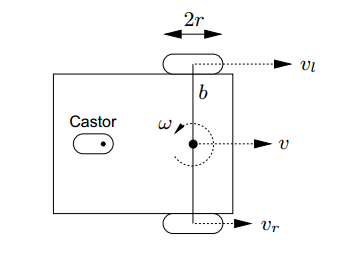
\includegraphics[width=6cm]{./imagenes/robot_diferencial.png}
\caption{Robot diferencial. }%\cite{pathfoll} .}
\label{fig:robot_diferencial}
\end{figure}


%
%Tomando en cuenta \cite{pathfoll}, si modelamos la línea detectada como una recta, la situación geométrica del problema se asemeja a la mostrada en la figura \ref{fig:sistema1}.
%
%\begin{figure}[h]
%\centering
%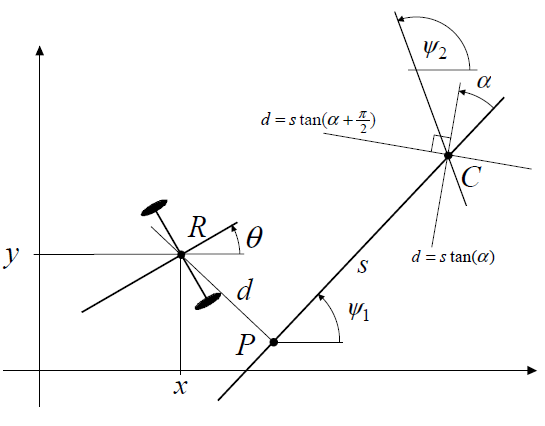
\includegraphics[width=10cm]{./imagenes/sistema1.png}
%\caption{Gráfico de la línea a seguir y del robot según \cite{pathfoll}.}
%\label{fig:sistema1}
%\end{figure}
%
%
%Las ecuaciones de velocidad para este problema según \cite{pathfoll} son:
%
%\begin{equation}
%\dot{s}=v \cos (\theta - \Psi)
%\end{equation}
%
%\begin{equation}
%\dot{d}=v \sin (\theta - \Psi)
%\end{equation}
%
%\begin{equation}
%\dot{\theta}=\omega  
%\end{equation}
%
%Donde v y $\omega$ son las velocidades lineal y angular del punto medio entre las ruedas, C.
 Si los motores se mueven a velocidades $\omega_R$ y $\omega_L$, estás velocidades son \cite{planning}:

\begin{equation}
v=\frac{r(\omega _R + \omega _L)}{2}
\end{equation}


\begin{equation}
\vert \omega_{C} \vert	=\frac{ \vert r(\omega _R - \omega _L) \vert }{L}
\end{equation}

Donde L es la distancia entre las ruedas. 

\subsubsection{Modelado 1}
Se toma como hipótesis que el vehículo se encuentra siempre sobre la linea a seguir.  Por lo que la señal de error se toma como la distancia entre el centro de la línea de sensores y el punto de intersección entre la línea de sensores y la recta a seguir. Esta situación se muestra en la figura \ref{fig:carrito1}.

\begin{figure}[h]
\centering
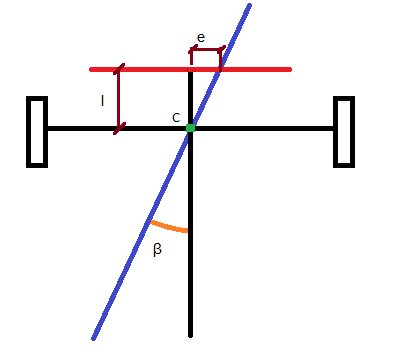
\includegraphics[width=10cm]{./imagenes/carrito1.png}
\caption{Esquema del robot sobre la línea a seguir (azul). La línea roja representa la línea de sensores, $e$ es la distancia medida entre el centro de los sensores y la intersección de la recta a seguir con la línea de los sensores, y $\beta $ es el ángulo entre la línea a seguir y el eje central del robot.}
\label{fig:carrito1}
\end{figure}

Tomando las ecuaciones anteriores como referencia, las velocidades en módulo serían:

\begin{equation}
\dot{\beta}=\omega_C
\end{equation}

Dado que sólo poseemos la medición de $e$, se propone la siguiente estrategia para la medición del ángulo. Suponemos que el punto centro entre las dos ruedas se mantiene siempre sobre la línea a seguir. Bajo esta suposición, podemos calcular $\beta $ por trigonometría:

\begin{equation}
\tan(\beta)=\frac{e}{l}
\end{equation}
Redaccion 1:\\
Como $l$ es fijo, la medición de $e$ puede traducirse en una medición del ángulo. Así, de esta manera, podríamos buscar minimizar el ángulo para alinear el robot con la pista. Como la medición se hace suponiendo que C está sobre la línea , si el robot no está centrado respecto a la pista el cálculo del ángulo va a indicar una medición errónea (ya que la suposición de que $\beta=\theta$ no es válida), por lo que al llevar a cero el $ \beta $ medido de esta manera se termina garantizando que el robot esté centrado respecto a la pista.

Redaccion 2:\\
Como $l$ es fijo, y $e$ es lo que el sensor de linea mide, se puede calcular el valor de $\beta$. De esta manera, se podría buscar minimizar este angulo, considerando que $\beta$ es la medición de la orientación del robot en el espacio, es decir $\beta \approx \theta$. Esta hipótesis sera valida siempre y cuendo el centro del dispositivo este sobre la linea. Suponer esto tiene sentido siempre y cuendo todo el sistema controlado sea lo suficientemente rápido y preciso para corregir cualquier perturbación antes de que el centro se desplace y eche por tierra el modelado del sistema.

Bajo estas simplificaciones, nos basta con mirar el comportamiento de $\beta$:

\begin{equation}
\dot{\beta}=\vert \omega_C \vert	=\frac{ \vert r(\omega _R - \omega _L) \vert }{L}
\end{equation}

Como sólo nos interesa la diferencia entra velocidades angulares del motor, se puede mantener $v$ constante tomando:

\begin{equation}
\omega _R = \omega _{fijo} + \frac{\Delta \omega}{2} 
\end{equation}

\begin{equation}
\omega _L = \omega _{fijo} -\frac{\Delta \omega}{2}
\end{equation}

Esto disminuiría el problema a una sola señal de control, $\Delta \omega$. Restaría realizar un análisis mas profundo sobre la dinámica de $e$.
Suponiendo el esquema de la figura \ref{fig:carrito1}, pero con un sensor de linea radial centrado en el centro con radio $T$ (como se ve en la figura...) resulta
% y disminuiría los efectos alineales influyendo sobre $\dot{e} $ sin embargo, como no se está tomando en cuenta la dinámica de e, no se tiene claro si esta restricción es necesaria. Se necesitaría profundizar en el análisis para poder asegurarlo.
\begin{equation}
e=T \sin (\beta)  \Longrightarrow \dot{e}=T \cos (\beta) \dot{\beta}  \Longrightarrow \dot{e} = T \omega \cos(\beta)
\end{equation}

si $\vert\beta\vert<10^o$ resulta que  
\begin{equation}
\dot{e} = T \omega \quad \wedge \quad  e=T \beta
\end{equation}

En caso de que esta suposición no se cumpla entraran en juego las no linealidades antes vistas.

\subsubsection{Radio de giro}
Cuando el robot gira siguiendo una curva la disposición es como se muestra en la siguiente figura:
En la figura \ref{fig:girando} se muestra la disposicion del robot cuando esta siguiendo una curva.
\begin{figure}[h]
\centering
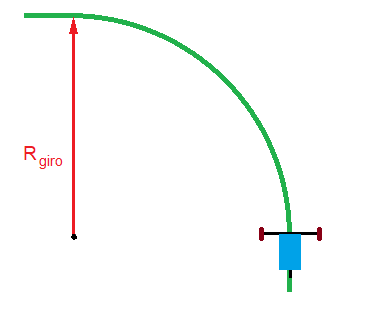
\includegraphics[width=10cm]{./imagenes/carrito_girando.png}
\caption{esquema del robot girando.}
\label{fig:girando}
\end{figure}

En este caso la velocidad del punto  C (punto medio entre las dos ruedas del robot) tiene una componente tangencial, v, y una componente de giro, $\omega$, dadas por: 

\begin{equation}
v =\frac{r(\omega _R + \omega _L) }{2}=r \omega_{fijo}
\end{equation}

\begin{equation}
\omega_{C} =\frac{r(\omega _R - \omega _L) }{L}= \frac{  r \Delta \omega} {L}
\end{equation}

Como la relación entre ambas magnitudes es:


\begin{equation}
v=R_{giro} \omega_{C}
\end{equation}

obtenemos:
\begin{equation}
\Delta \omega= \frac{\omega_{fijo}L}{R_{giro}}
\end{equation}

Así, mientras más pequeño sea el radio de giro, más grande debe ser $\Delta \omega$.


%Redaccion anterior
%Así, mientras más pequeño sea el radio de giro, más grande debe ser $\Delta \omega$ . Si definimos que $\omega _{fijo}=300 rpm $, para obtener un radio de giro mínimo de 1,5 veces R necesitaríamos $\Delta \omega =100 rpm $, mientras que para uno igual a R necesitaríamos $\Delta \omega =150 rpm $.

\section{Modelado de los motores}
Según \cite{alex} se puede modelar el motor según la siguiente ecuación diferencial:
\begin{equation}
J\ddot{\theta}=\frac{k_2}{R}V_i-\frac{k_2 k_2}{R} \dot{\theta}-k_3\dot{\theta} 
\end{equation}
donde $k_1$ es la constante que relaciona la fuerzamagneto motriz con la velocidad angular; $k_2$ relaciona la cupla motora con la corriente; $k_3$ relaciona la velocidad angular con el torque de fricción; $R$ es la resistencia del bobinado; $J$ es el momento de inercia del eje y $V_i$ es la tension entre los bornes del motor.
La función de transferencia entonces resulta
\begin{equation}
\frac{\theta}{V_i}=\frac{k_2}{Rs(sJ+\frac{k_2k_1}{R}+k_3)}
\end{equation}

considerando que $\theta$ es proporcional al desplazamiento del dispositivo $x$ y $V_i$ es proporcional a la señal de control, simplificando resulta:
\begin{equation}
\frac{\theta}{V_i}=\frac{k_2/{JR}}{s(s+\frac{k_2k_1}{JR}+ \frac{k_3}{J} )}
\end{equation} 
escribiendo genéricamente 
\begin{equation}
\frac{\theta}{V_i}=\frac{a}{s(s+b)}
\end{equation}
 donde a y b son parámetros a determinar. Por cuestiones de practicidad (segun tania) en vez de usar $\theta$ se usa $\dot{\theta}$ , lo que produce la siguiente funcion de transferencia
 \begin{equation}
 \frac{\omega}{V_i}=\frac{a}{(s+b)}
 \end{equation}
 
 \section{Modelado de los motores2 }
 
 Según \cite{dorf} la función de transferencia de la combinacion motor-carga despreciando el torque de la perturbacion resulta
 \begin{equation}
 \frac{\theta(s)}{V_f(s)}=\frac{K_m}{s(Js+b)(L_fs+R_f)}
 \end{equation}
 donde $\theta$ es la posición angular,$V_f$ es la tension de exitacion, $K_m$ es la constante que relaciona la corriente con el par del motor, $J$ es el momento de inercia del eje, $b$ es la constante de friccion del eje, $L_f$  y $R_f$ es la autoinductancia y resistencia del bobinado. Simplificando la función de transferencia resulta
 \begin{equation}
 \frac{\theta(s)}{V_f(s)}=\frac{k}{s(s+a)(s+b)}
 \end{equation}
 donde $k$,$a$,$b$ son constantes a determinar mediante la identificación.\\
 Por practicidad en vez de usar $\theta$ se usa $\dot{\theta}$, lo que produce la siguiente funcion de transferencia
 \begin{equation}
 \frac{\dot{\theta}(s)}{V_f(s)}=\frac{k}{(s+a)(s+b)}
 \end{equation}
  
\section{Sistema de medición de RPM y sensores de linea}

\section{Obtención de los parámetros}

\section{Ajuste fallido por medio de Z-N}
Explicar que es un controlador PID antes. Lo que sigue es un choreo del ogata\\

Según \cite{ogata} como casi todos los controladores PID se ajustan en el sitio, en la literatura se han propuesto muchos tipos diferentes de reglas de sintonización, que permiten llevar a cabo una sintonización delicada y fina de los controladores PID en el sitio. Asimismo, se han desarrollado métodos automáticos de sintonización y algunos de los controladores PID poseen capacidad de sintonización automática en línea. Actualmente se usan en la industria formas modificadas del control PID, tales como el control I-PD y el control PID con dos grados de libertad.

La utilidad de los controles PID estriba en que se aplican en forma casi general a la mayoría de los sistemas de control. En particular, cuando el modelo matemático de la planta no se conoce y, por lo tanto, no se pueden emplear métodos de diseño analíticos, es cuando los controles PID resultan más útiles. En el campo de los sistemas para control de procesos, es un hecho bien conocido que los esquemas de control PID básicos y modificados han demostrado su utilidad para aportar un control satisfactorio, aunque tal vez en muchas situaciones específicas no aporten un control óptimo.

Las reglas de Ziegler-Nichols son muy convenientes cuando no se conocen los modelos matemáticos de las plantas. Tales reglas sugieren un conjunto de valores de $K_p$, $T_i$ y $T_d$ que darán una operación estable del sistema. No obstante, el sistema resultante puede presentar una gran sobreelongación en su respuesta escalón de forma que resulte no aceptable. En tales casos se necesitará una serie de ajustes finos hasta que se obtenga el resultado deseado. De hecho, las reglas de sintonía de Ziegler-Nichols dan una estimación razonable de los parámetros del controlador y proporcionan un punto de partida para una sintonía fina, en lugar de dar los parámetros $K_p$, $T_i$ y $T_d$ en un único intento.

Tal determinación de los parámetros de los controladores PID o sintonía de controladores PID se pueden realizar mediante experimentos sobre la planta. Hay dos métodos denominados reglas de sintonía de Ziegler-Nichols: método de la respuesta al esalón y método del $K_{inestable}$.  

\subsection{Metodo de Z-N: respuesta al escalón}
Esto esta sacado del PDF que nos paso COLON:\\

Según \cite{biblia_PID} este método se basa en registrar la respuesta a un escalón
unitario del sistema a lazo abierto, para luego ajustar los tres parámetros de un modelo
de primer orden con retardo dado por la ecuación \ref{eq:ajusteZN}.

\begin{equation}
G_s(s)=\frac{K_p}{Ts+1}e^{-sL}
\label{eq:ajusteZN}
\end{equation}


\begin{figure}[h]
\centering
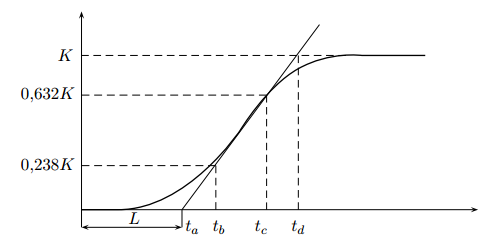
\includegraphics[width=10cm]{./imagenes/escalon_z-n.png}
\caption{Determinación gráfica de los parámetros de un modelo a partir de
la respuesta escalón en forma de S}
\label{fig:escalon_zn}
\end{figure}




Los parámetros del modelo de la ecuación \ref{eq:ajusteZN} pueden ser determinados por medio de la figura \ref{fig:escalon_zn}. La ganancia estática $K$ la obtenemos del valor final de la salida del proceso dividido el valor máximo de la entrada. 

Para hallar los otros dos parámetros hay varias alternativas. Una de ellas consiste en trazar una recta tangente al punto donde de la respuesta al escalón presenta la mayor pendiente. El valor de la demora $L$ lo obtenemos de la intersección de esta recta con el eje horizontal. El valor de la constante de tiempo $T$ lo podemos obtener a partir de la distancia $t_a-t_c $, donde $t_c$ es el tiempo donde la respuesta al escalón es $0.632K$.
Otro método, un poco más preciso, consiste en determinar los puntos $t_b$ y $t_c$ donde $s(t)$ toma los valores $0.283K$ y $0.632K$, respectivamente. Luego, la demora y la constante de tiempo la hallamos a partir de la ecuación \ref{eq:calculo_T_L}

\begin{equation}
T=1.5(t_c -t_b) \quad	L=t_c-T
\label{eq:calculo_T_L}
\end{equation}




\section{Datos medidos}
Respuesta escalón motores


\begin{figure}[h]
\centering
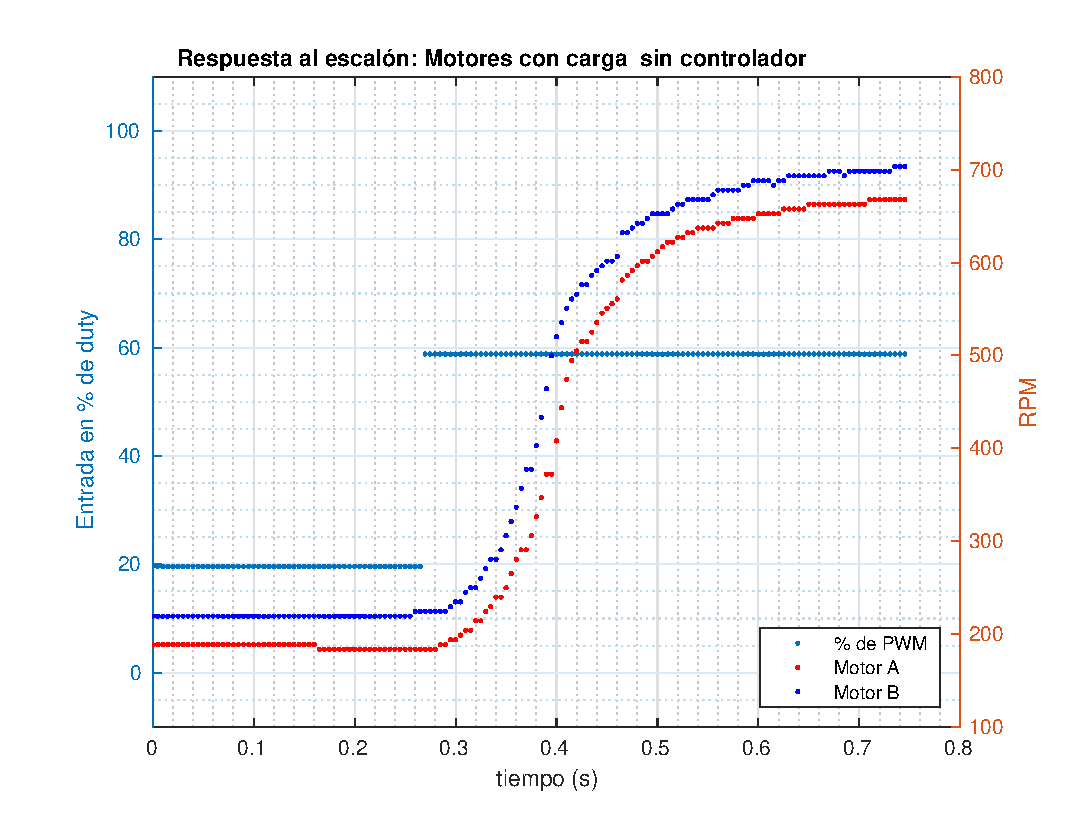
\includegraphics[width=15cm]{./imagenes/resp_escalon_motores_2}
\end{figure}
Motor A:
\begin{equation}
M_a(s)= \frac{7075.3 e^{-0.013s}}{(s+9.631)(s+67.5)}
\end{equation}
Controlador A:
\begin{equation}
C_a(s)= \frac{  19.243 (s-11.74)}{s}
\end{equation}


Motor B
\begin{equation}
M_b(s)= \frac{5042.1 e^{-0.013s}}{(s+9.988) (s+45.48)}
\end{equation}

Controlador B

\begin{equation}
C_b(s)= \frac{ 18.68 (s-10.93)}{s}
\end{equation}


Se ajustaron ambos motores para que con el controlador tengan una respuesta identica, la respuesta a lazo cerrado es:
\begin{figure}[h]
\centering
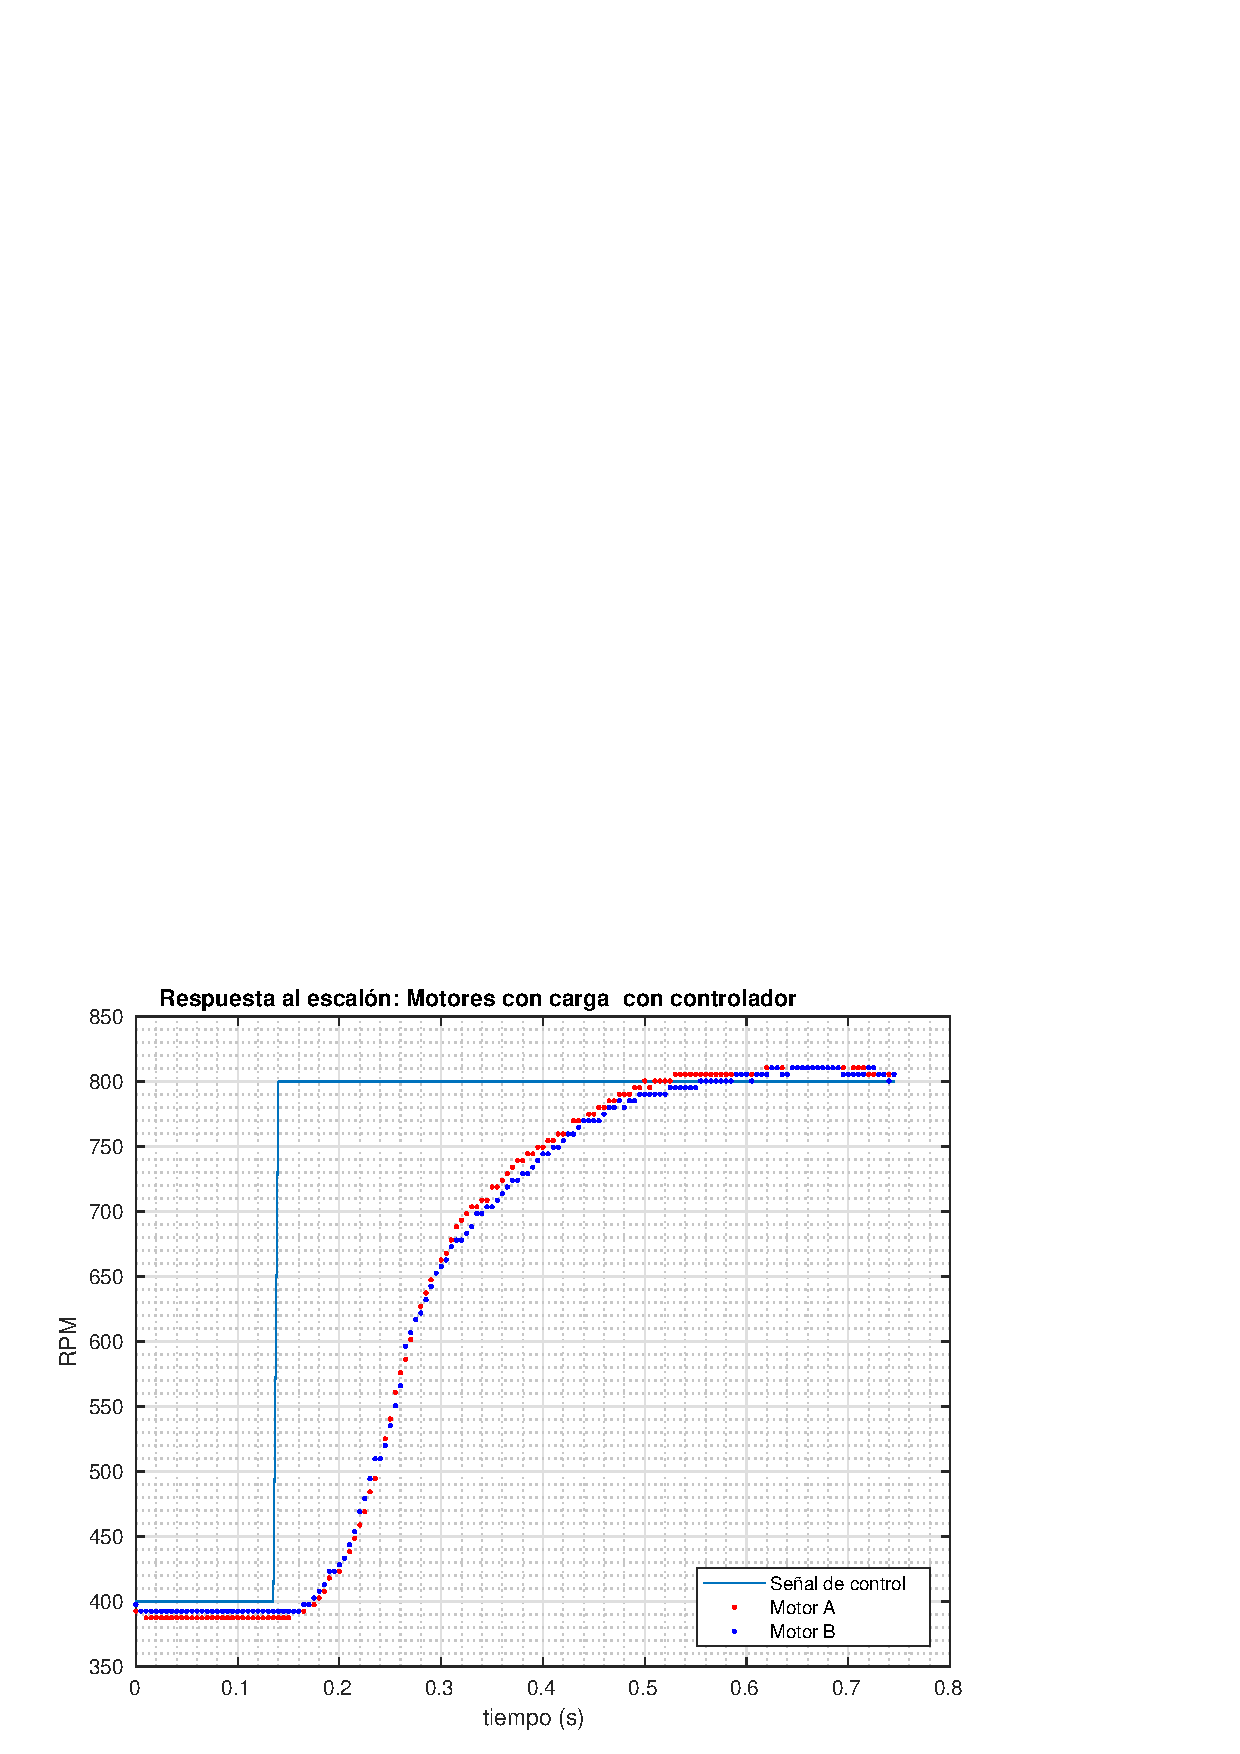
\includegraphics[width=15cm]{./imagenes/resp_escalon_motores_controlados_2}
\end{figure}

\section{Ensayo al Escalón}

En función de lo analizado anteriormente, podemos pensar que si el robot arranca alineado con una línea recta, y manteniendo la restricción de v constante, entonces la planta se comporta como un sistema cuya entrada es $\Delta \omega$ y su salida $\beta $, gobernado por la ecuación:

\begin{equation}
\dot{\beta}= \frac{r\Delta\omega}{L} 
\label{eq:sys_tot_teo} 
\end{equation}

Para realizar el ensayo al escalón se debería empezar con $\Delta \omega = \beta = \theta=0$  y luego cambiar $\Delta \omega$  abruptamente a un valor final ($\Delta \omega$  es el escalón de entrada) midiendo el valor de $\beta$ obtenido. Físicamente esto implica que el robot debe empezar andando a velocidad constante, perfectamente alineado con la línea, y luego girar hasta perder la línea (más allá de este punto no tiene sentido seguir porque se pierde la medición).
Si el cambio de velocidad de los motores fuese automático, el robot giraría siguiendo una circunferencia perfecta como se ve a en la figura \ref{fig:carritoEsc}.

\begin{figure}[h]
\centering
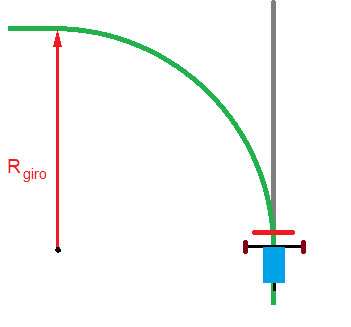
\includegraphics[width=10cm]{./imagenes/carrito_Ensayo_escalon.png}
\caption{Trayectoria seguida por el robot si empieza a girar a $\Delta \omega $ constante (verde) arrancando inicialmente alineado con la línea (gris).}
\label{fig:carritoEsc}
\end{figure}
%Lo que nos interesa es saber cuánto tiempo transcurre hasta que pierde la línea. Dicho punto sería cuando el último sensor de la derecha está sobre la línea verde. Si la distancia entre el eje central del robot y éste LED es $d_1$, entonces el LED se desplaza siguiendo una trayectoria circular de radio $R_{giro}$+$d_1$ …..
%Terminar de poner ideas para el cálculo
%Borrador:


\section{Ensayo escalón carrito implementación}

Necesidad de que el sistema sea lineal, esta es la respuesta de los motores en función de las RPM de entrada:

\begin{figure}[h]
\centering
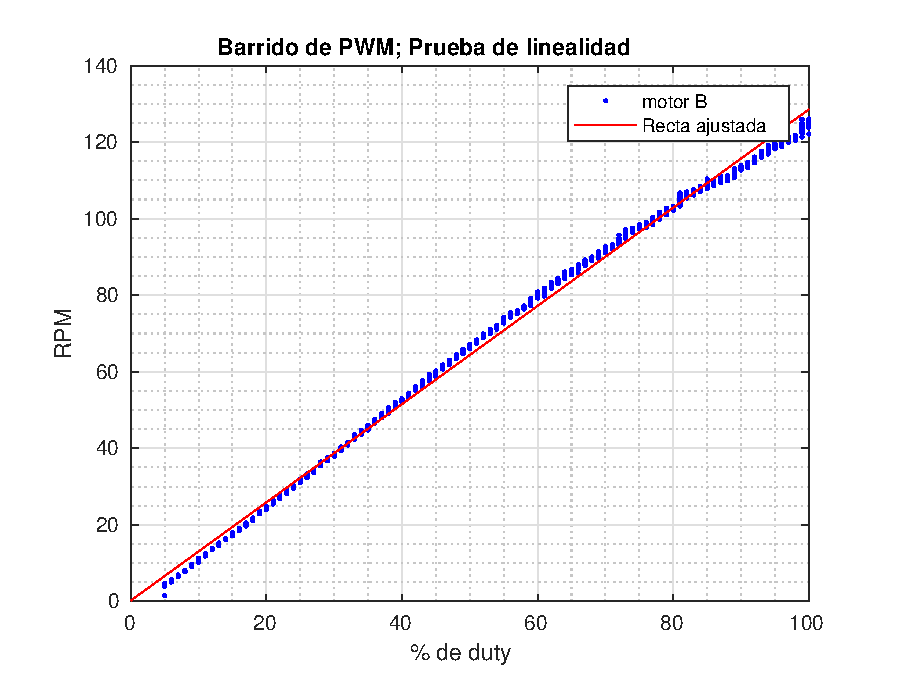
\includegraphics[width=10cm]{./imagenes/prueba_linealidad}
\caption{el error medio cuadrático del ajuste de la recta es de 2.0624. REVISAR ESTO; NO TIENE SENTIDO EL EJE Y, en otra imagen parece la palabra "frecuencia de giro" pero no tiene sentido.}
\label{fig:prueba_linealidad}
\end{figure}

Las consideración antes descriptas son válidas dentro de la región de linealidad del sistema. Como se vió anteriormente, es necesario que el dispositivo se encuentre centrado sobre la linea y moviendose a velocidad constante. 

El objetivo de esta etapa es obtener el modelo del sistema; Dadas algunas complicaciones practicas, se implemento un controlador proporcional ajustado experimentalmente para que las hipótesis de que el vehiculo se encuentre centrado sobre la linea y moviendose sean lo mas "validas posibles". 

Un ensayo modelo se muestra a continuacion:
\begin{figure}[h]
\centering
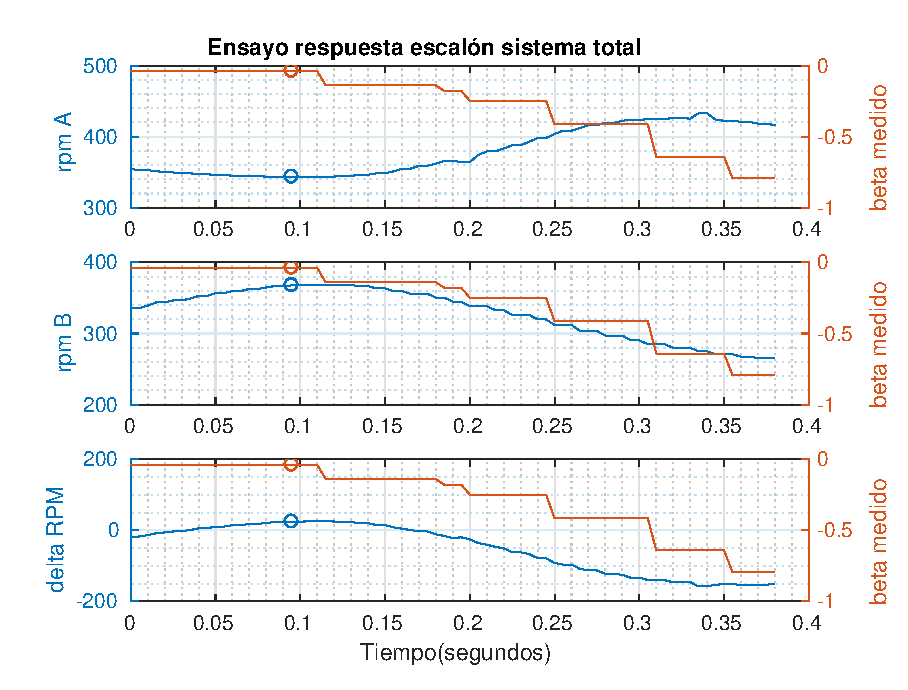
\includegraphics[width=10cm]{./imagenes/resp_escalon_sys_total}
\caption{El circulo marca cuando se desactiva el control y el sistema comienza a trabajar en lazo abierto. En esta caso $\Delta \omega=-50 $ RPM}
\label{fig:ens_esc_syst}
\end{figure}

Para un conjunto de estos ensayos se estimo el siguiente sistema:
\begin{equation}
Sys_{tot}= \frac{0.028934}{s}  
\label{eq:sys_tot_est}
\end{equation}

De la ecuación \ref{eq:sys_tot_teo} y de \ref{eq:sys_tot_est}  se concluye que $\frac{2r}{R}=0.028934 $ siendo que los parámetros medidos son $r=1.5cm$ y $R=16cm$, lo cual da $\frac{r}{R}=0.09375 $. Esta discrepancia no se pudo explicar aún.   

\section{Sistema total y control}

Si se parte de la suposición de que los motores se comportan de manera semejante, el diagrama del sistema total resulta:


\begin{figure}[h]
\centering
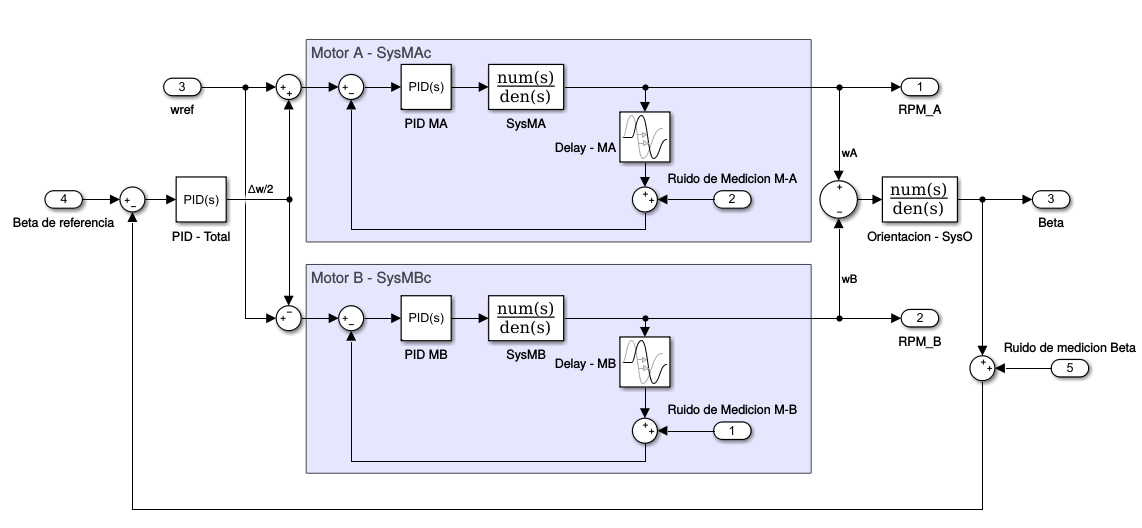
\includegraphics[width=10cm]{./imagenes/sistema_total}
\caption{}
%\label{}
\end{figure}


A la hora de implementar el control se encontraron varios inconvenientes.... Poner Z-N, problemas de rozamiento y de inestabilidad; falta de linealidad a bajas RPM


\begin{thebibliography}{X}
%\bibitem{Farmers}Bergerman, M., Maeta, S. M., Zhang, J., Freitas, G. M., Hamner, B., Singh, S., \& Kantor, G. (2015). Robot farmers: Autonomous orchard vehicles help tree fruit production. IEEE Robotics \& Automation Magazine, 22(1), 54-63.
%\bibitem “Path Following Mobile Robot in the Presence of Velocity Constraints”, Bak, Poulsen y Ravn.
%\bibitem “Robotics: Modelling, Planning and Control”, Siciliano, Sciavicco, Villani y Oriolo.
\bibitem{lambo} \url{http://lamborghino.com}. 
\bibitem{motores}\url{https://www.pololu.com/product/3061}
\bibitem{puenteH}\url{ https://www.pololu.com/file/0J86/TB6612FNG.pdf}
\bibitem{arduinoNano} \url{https://store.arduino.cc/usa/arduino-nano}
\bibitem{pathfoll} \textit{Path Following Mobile Robot in the Presence of Velocity Constraints}, Bak, Poulsen y Ravn.
\bibitem{planning} \textit{Robotics: Modelling, Planning and Control}, Siciliano, Sciavicco, Villani y Oriolo.
\bibitem{alex} Tesis de alexei.
\bibitem{dorf} Dorf 10ma edicion; pagina 58.
\bibitem{paginaZN} \url{https://sites.google.com/site/picuino/ziegler-nichols}.
\bibitem{ogata} Ogata 5ta edicion capitulo 5
\bibitem{biblia_PID} PID que nos paso colon.
\bibitem{paginaPID}\url{https://sites.google.com/site/picuino/ziegler-nichols}
\end{thebibliography}
%Referencias
%[1]: “Path Following Mobile Robot in the Presence of Velocity Constraints”, Bak, Poulsen y Ravn.
%[2]: “Robotics: Modelling, Planning and Control”, Siciliano, Sciavicco, Villani y Oriolo.



\end{document}











\section{BIBLIOGRAFÍA ORIENTATIVA}

Paginas
\begin{itemize}
\item http://www.nongnu.org/avr-libc/
\item https://www.microchip.com/webdoc/AVRLibcReferenceManual/index.html
\item http://www.microchip.com/mplab/mplab-x-ide
\item https://garretlab.web.fc2.com/en/arduino/inside/index.html
\end{itemize}
%\nocite{*}  % Es para agregar toda la bibliografia de manera indiscriminada. 
\bibliographystyle{ieeetr}
%\nocite{PainaCareli}
%\nocite{nvidia2011nvidia}
%\nocite{bradski2008learning}
%\nocite{bishop2006pattern}
%\nocite{Stereolabs}
%\nocite{quigley2009ros}
%\nocite{jetson}
%\nocite{scaramuzza2011visual}
%\nocite{fraundorfer2012visual}


%\bibliography{biblioteca_plan}

%\begin{thebibliography}{X}
%\bibitem{Paina}Auat Cheein, F. A., Steiner, G., Perez Paina, G., \& Carelli, R. (2010). Aplicación de un EIF-SLAM en entornos agrícolas basado en detección de troncos de árboles.
%\bibitem{Farmers}Bergerman, M., Maeta, S. M., Zhang, J., Freitas, G. M., Hamner, B., Singh, S., \& Kantor, G. (2015). Robot farmers: Autonomous orchard vehicles help tree fruit production. IEEE Robotics \& Automation Magazine, 22(1), 54-63.
%
%%\bibitem{libros} Salazar, M.G. and Barahona, M.L. (2017). Methods in Engineering. Prentice Hall, Englewood Cliffs, NJ, USA.
%%\bibitem{revistas}Choleski,   R.L.   and   Kutta,   S.H.   (1982).   Reduced   noise and quadratic problem. Eng., v. 8, n. 3, p. 409-428.
%%\bibitem{congreso}Choleski,   R.L.   and   Kutta,   S.H.   (2002). Optimum design. Proceeding Electronic Congress, New York, May. % conferencias y seminarios
%%\bibitem{Tesis} Marcos,  A.  (2003). Evaluación de sistemas dinámicos.  Tesis doctoral, Universidad Nacional de Colombia. %o disertasiones
%%\bibitem{documento_tecnico} Marcos, A. (2004). Respuesta de modelos no lineales. Reporte Técnico Report B5875, Offshore Technology Research Center, USA.% o repores
%\end{thebibliography}




\end{document}
